\documentclass{beamer}


\makeatletter
\newcommand*\Alt{\alt{\Alt@branch0}{\Alt@branch1}}

\newcommand\Alt@branch[3]{%
  \begingroup
  \ifbool{mmode}{%
    \mathchoice{%
      \Alt@math#1{\displaystyle}{#2}{#3}%
    }{%
      \Alt@math#1{\textstyle}{#2}{#3}%
    }{%
      \Alt@math#1{\scriptstyle}{#2}{#3}%
    }{%
      \Alt@math#1{\scriptscriptstyle}{#2}{#3}%
    }%
  }{%
    \sbox0{#2}%
    \sbox1{#3}%
    \Alt@typeset#1%
  }%
  \endgroup
}

\newcommand\Alt@math[4]{%
  \sbox0{$#2{#3}\m@th$}%
  \sbox1{$#2{#4}\m@th$}%
  \Alt@typeset#1%
}

\newcommand\Alt@typeset[1]{%
  \ifnumcomp{\wd0}{>}{\wd1}{%
    \def\setwider   ##1##2{##2##1##2 0}%
    \def\setnarrower##1##2{##2##1##2 1}%
  }{%
    \def\setwider   ##1##2{##2##1##2 1}%
    \def\setnarrower##1##2{##2##1##2 0}%
  }%
  \sbox2{}%
  \sbox3{}%
  \setwider2{\wd}%
  \setwider2{\ht}%
  \setwider2{\dp}%
  \setnarrower3{\ht}%
  \setnarrower3{\dp}%
  \leavevmode
  \rlap{\usebox#1}%
  \usebox2%
  \usebox3%
}
\makeatother

\usetheme[block=fill]{metropolis}




\usepackage[utf8]{inputenc}
\usepackage[T1]{fontenc}
\usepackage[english]{babel}

\usepackage{amsmath}
\usepackage{tikz}
\usepackage{mathrsfs}



\newcommand{\R}{\ensuremath{\mathbb{R}}}
\newcommand{\Rb}{\ensuremath{\overline{\mathbb{R}}}}
\newcommand{\N}{\ensuremath{\mathbb{N}}}
\newcommand{\Q}{\ensuremath{\mathbb{Q}}}
\newcommand{\Z}{\ensuremath{\mathbb{Z}}}
\newcommand{\C}{\ensuremath{\mathbb{C}}}
\newcommand{\U}{\ensuremath{\mathbb{U}}}
\newcommand{\F}{\ensuremath{\mathbb{F}}}
\newcommand{\K}{\ensuremath{\mathbb{K}}}
\newcommand{\TODO}{\textbf{TODO}}


\newcommand\eqdef{\stackrel{\mathclap{\mbox{\tiny def}}}{=}}


\newcommand{\ket}[1]{|#1\rangle}
\newcommand{\bra}[1]{\langle#1|}
\newcommand{\braket}[2]{\langle#1|#2\rangle}

\newcommand{\dd}{\mathrm{d}}
\newcommand{\der}[2]{\frac{\dd{#1}}{\dd{#2}}}
\newcommand{\dern}[3]{\frac{\dd^{#3} #1}{\dd{#2}^{#3}}}
\newcommand{\dpar}[2]{\frac{\partial{#1}}{\partial{#2}}}
\newcommand{\dparn}[3]{\frac{\partial^{#3} {#1}}{\partial{#2}^{#3}}}


\newcommand{\mat}[1]{\begin{pmatrix}#1\end{pmatrix}}
\newcommand{\bs}{\boldsymbol}

\newcommand{\Tr}{\mathsf{Tr}\,}
\newcommand{\argmin}{\mathop{\mathsf{arg\,min}}}
\newcommand{\rk}{\mathsf{rk}\,}
\newcommand{\diag}{\mathsf{diag}\,}


\newcommand{\class}[1]{{\mathscr{C}^{#1}}}

\newcommand{\trnorm}[1]{\frac{#1}{\Tr\left({#1}\right)}}
\newcommand{\ml}{_{M\!L}}


\newcommand{\maxim}[3]{\begin{cases}
    \mathbf{maximize}\,\quad #1& \mathbf{on}\; #2\\
    \mathbf{subject\;to}\quad #3
  \end{cases}}
\newcommand{\maximf}[2]{\begin{cases}
    \mathbf{maximize}\,\quad #1& \mathbf{on}\; #2
  \end{cases}}
\newcommand{\maxima}[3]{\begin{cases}
    \mathbf{maximize}\,\quad #1& \mathbf{on}\; #2\\
    \mathbf{subject\;to}\quad \begin{aligned}[t]#3\end{aligned}
  \end{cases}}

\newcommand{\minim}[3]{\begin{cases}
    \mathbf{minimize}\;\,\quad #1& \mathbf{on}\; #2\\
    \mathbf{subject\;to}\quad #3
  \end{cases}}
\newcommand{\minimf}[2]{\begin{cases}
    \mathbf{minimize}\,\quad #1& \mathbf{on}\; #2
  \end{cases}}
\newcommand{\minima}[3]{\begin{cases}
    \mathbf{minimize}\;\,\quad #1& \mathbf{on}\; #2\\
    \mathbf{subject\;to}\quad \begin{aligned}[t]#3\end{aligned}
  \end{cases}}

\newcommand{\gap}{\hspace{0.8cm}}
\newcommand{\twoline}{\vphantom{\frac\int\int}}
\graphicspath{{../img/}}




\title{Error estimation in maximum likelihood reconstruction for
    quantum state tomography}
\author{Thibaut Pérami}
\institute{LKB, Collège de France}
\date{September 11, 2019}

\begin{document}

\maketitle

\begin{frame}{Quantum state tomography}
  Experiment --> Lots of data -> Statistics --> estimated/reconstructed state
  --> Expectation of function of state

  |--> Variance of function of state
\end{frame}

\section{Setup and Goal}


\begin{frame}{The experimental setup}
  Simply the experiment diagram
\end{frame}

\begin{frame}{The goal$\colon{}$ Create a Maxwell demon}
  Study how an atom can give heat to a hotter cavity.
  Diagram with and without demon
\end{frame}

\section{Atoms and light in cavities}

\begin{frame}{Circular Rydberg atoms}

  \begin{itemize}
  \item exited state $\ket e$ \TODO{} tikz with 51 and 54 and n=?, l=m=n
  \item exited state $\ket g$
  \item exited state $\ket f$
  \end{itemize}

  \begin{block}{Hamiltonian}
    \[H = \frac{\hbar \omega}2 \sigma_Z\]
  \end{block}

\end{frame}

\begin{frame}{Rydberg atoms in a classical field: Rabi oscillation}
  \[H = \frac{\hbar \omega}2 \sigma_Z \pause - \bs D \cdot \bs E\]

  \pause{}

  \begin{block}{Secular approximation in interaction picture: Rabi oscillation}
    \[H_1 = \frac{\hbar \Delta_r}2 \sigma_Z - \frac{\hbar \Omega_r}2
      \mat{0&e^{i\phi}\\e^{-i\phi}&0} = \frac{\hbar \Omega_r'}2 \bs \sigma
      \cdot \bs n\]
  \end{block}

  \pause{}

  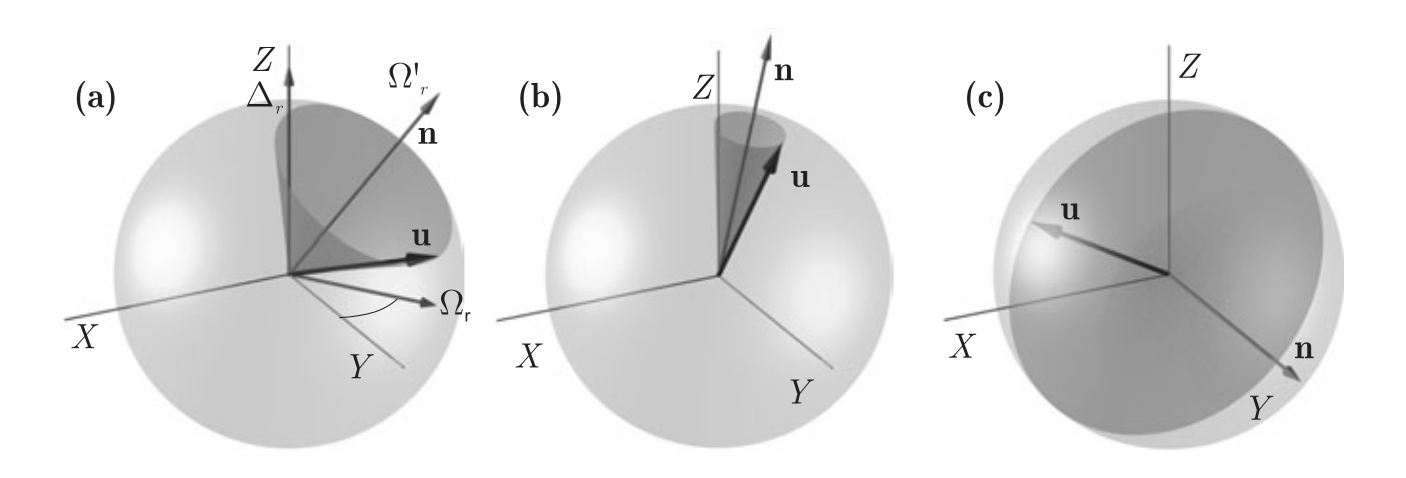
\includegraphics[width=\textwidth]{Rabi.png}
\end{frame}

\begin{frame}{EM field in a resonant cavity}

  \[H = \hbar\omega \left(N +\frac12\right)\]
\end{frame}

\begin{frame}{Rydberg atom in a resonant cavity}
  f
\end{frame}



\section{Maximum likelihood estimation}

\begin{frame}{Estimation theory}

  \begin{block}{Goal}
    Estimating parameter $\theta$ for observation $X$ and law $P_\theta(X = x)$
  \end{block}

  \pause{}

  \begin{block}{Estimator}
    deterministic function $\hat \theta(x)$ such that $P_\theta(\hat \theta(X)
    \approx \theta)$ is high
  \end{block}

  \pause{}

  \begin{block}{Likelihood}
    \[P_\theta(A) = \int_A \mathcal{L}_x(\theta) \dd x\]
    \[\ell_x = \log \mathcal{L}_x\]
  \end{block}
  
\end{frame}

\begin{frame}{Fischer information and Cramér-Rao bound}
  Light and fast 30s
\end{frame}

\begin{frame}{MaxLike estimation}
\end{frame}



\section{Density matrices}

\begin{frame}{Probability distribution on quantum states}
  \[\int_S \bra \psi A\ket \psi \dd P(\psi)\pause = \int_S \Tr\big(A\ket \psi \bra \psi\big) \dd
    P(\psi) \pause = \Tr\left(A \int_S\ket \psi \bra \psi \dd P(\psi) \right)\]
  \pause{}
  \begin{block}{Density matrix, $\mathcal{D}(\mathcal{H})$}
    \[\rho = \int_S\ket \psi \bra \psi \dd P(\psi)\]
  \end{block}

  \pause{}

\begin{itemize}
  \item[--] $\rho \geqslant 0$
    \pause{}
  \item[--] $\Tr \rho = 1$
    \pause{}
  \item[--] $\rho = \sum p_i \ket {\psi_i} \bra{\psi_i}$
\end{itemize}

  \pause{} \vspace{3mm}

\begin{block}{Pure states}
  $P(\psi) = 1 \iff \rho = \ket \psi \bra \psi \iff \Tr(\rho^2) = 1 \iff \rk
  \rho = 1$.
\end{block}
\end{frame}

\begin{frame}{The qubit}
  \TODO{} Nice diagram. Skip?
\end{frame}

\begin{frame}{Partial Trace}
  \TODO{}
\end{frame}



\section{Quantum operations}

\begin{frame}{Generalized measurement}
\end{frame}

\begin{frame}{Quantum operation}
\end{frame}

\begin{frame}{Krauss operators}
  Krauss theorem
\end{frame}

\begin{frame}{Likelihood with quantum operations}
\end{frame}

\newcommand{\pr}{_{||}}
\newcommand{\inv}{^{-1}}
\begin{frame}{Evaluation of observable on the estimator}

  \begin{center}
    \Large observable A on $\rho\ml$
  \end{center}

  \pause{}

  \begin{block}{Expectation}
    \[E_A = \Tr(\rho\ml A)\]
  \end{block}

  \pause{}

  \begin{block}{Variance}
    \[V_A = \Tr(A\pr \mathbb H\inv(A\pr))\]
    \begin{itemize}
    \item[--] $A\pr$ is $A$ projected on tangent space to $\mathcal{D}$ in $\rho\ml$
    \item[--] $\mathbb H$ is $\nabla^2f$ on the edge of $\mathcal{D}$ in
      $\rho\ml$:
      \[ \mathbb H(A) = \nabla^2 f\pr + \text{other term}\]
    \end{itemize}
  \end{block}
\end{frame}


\section{Convex Optimization}

\begin{frame}{Convex problem}
  \[\maxima{\Alt<1>f\ell(\Alt<1>x\rho)}{\Alt<1>x\rho}
    {\Alt<1>{g(x)}{\rho} &\geqslant 0\\ \Alt<1>{h(x)}{\Tr \rho} &= \Alt<1>{0}{1}}\]
  \pause{}

  \pause{}\vfill

  \centering \Large
  This is \alert{tractable}

  \TODO{} Add convexity hypothesis
\end{frame}

\begin{frame}{Projected gradient ascent}

  \[\rho_{n+1} = P(\rho_n + t_n \nabla \ell)\]

  \pause{}\vfill

  \begin{block}{Step size}
    $t_n$ minimize 2$^{\text{nd}}$ order: $\ell (\rho_n + h) = \ell(\rho_n) + \nabla
    \ell \cdot h + \frac12 h \cdot \nabla^2 \ell \cdot h$
  \end{block}

  \pause{}

  \begin{block}{Projection}
    \onslide<4->{$M = UDU^\dagger$} \onslide<5->{, $D = \diag(d)$}
    \[P(M) = \onslide<4->{U}
       \onslide<5->{\diag\Big (}
       \argmin_{\Alt<-4>\rho x \in \Alt<-4>{\mathcal{D}}{\mathcal{P}}}
       \|\Alt<5>{d-x}{\Alt<-3>MD - \rho}\|^2
      \onslide<5->{\Big)}
      \onslide<4->{U^\dagger}\]
    \onslide<5-> where $\mathcal{P}$ is the probability simplex
  \end{block}
\end{frame}


\begin{frame}{KKT conditions}
  \[\maxima{\ell(\rho)}{\rho}
    {\rho &\geqslant 0\\ \Tr \rho &= 1}\]

\begin{block}{Lagrangian}
  \[\mathcal{L}(\rho,\mu,\lambda) = \ell(\rho) + \braket{\mu}{\rho} - \lambda\Tr\rho\]
\end{block}

    \pause{}

\begin{block}{KKT}
  \begin{itemize}
  \item[--] $\rho \in \mathcal{D}$
  \item[--] $\nabla \mathcal{L} = 0 \implies \nabla \ell = \lambda I - \mu$
    \pause{}
  \item[--] $\mu > 0$
  \item [--] $\braket{\mu}{\rho} = 0$
  \end{itemize}
\end{block}
\end{frame}






\section{Quantum thermodynamics}

\begin{frame}{Thermal state at Maxwell Boltzmann distribution}
  \[\zeta_\beta = \trnorm{{\exp(\beta H)}}\]
\end{frame}

\begin{frame}{Exact Protocol}
  Bring back the diagram of Luis

  \TODO{} Think about it.
\end{frame}


\begin{frame}{Quantum information theory}

  \begin{block}{Shanon entropy}
    \[H(p_1,\ldots,p_n) = \sum_i -p_i\log (p_i)\]

  \vspace{-0.2cm}

  \end{block}

  \pause{}

  \begin{block}{VonNeuman Entropy}

  \vspace{-0.3cm}

    \[S(\rho) = -\Tr(\rho\log \rho) = H(p_1,\ldots,p_n) \gap \left(\rho = \sum p_i
      \ket {\psi_i}\bra{\psi_i}\right)\]

  \vspace{-0.2cm}

  \end{block}

  \pause{}

  \begin{block}{Mutual Infomation}
    \[I_{A:B} = S(\rho^A) + S(\rho^B) - S(\rho^{AB})\]
  \end{block}

  \pause{}

  \begin{block}{Reltative entropy to $\zeta$ (Kullback–Leibler divergence)}
    \[D(\rho) = \Tr(\rho (\log \rho - \log \zeta))\]
  \end{block}
\end{frame}

\begin{frame}{New second laws of thermodynamics}

  \[  \onslide<2->{- \Delta I_{QC:D} +}\Delta\beta Q \mathrel{\Alt<3>=\geqslant}
    \Alt<-2>0{\Delta D_{QC}}\]

\end{frame}

\begin{frame}{Heat vs relative temperature}
  1 plot (maybe multiple ones)
\end{frame}



\section{Deviation computation}

\begin{frame}{Monte-Carlo algorithm}

  \vspace{0.5mm}

  \begin{block}{Input}
    $n$ probabilities $p_i$ with standard deviation $\Delta p_i$
  \end{block}

  \pause{}
  \begin{block}{Goal}
    Simulate a corresponding probability distribution
  \end{block}

  \pause{}
  \begin{block}{Difficulty}
    We must project and truncate the distribution $\prod_i
    \mathcal{N}(p_i,\Delta p_i)$ to the polyhedron $\mathcal{P}$ of valid probability distributions
  \end{block}

  \pause{}
  \emph{Hit and run Markov chain}
  \begin{itemize}
  \item[--] Take a random direction $d$
  \item[--] Compute the segment $S = \{x_n + t d\} \cap \mathcal{P}$
  \item[--] Project the distribution on that segment (it's a normal law)
  \item[--] Draw $x_{n+1}$ from that distribution
  \end{itemize}

\end{frame}

\begin{frame}{Expectation and variance\onslide<4>{, Asymptotics}}
  \[I_h\onslide<4>{(N)} = \int_{\rho \in \mathcal{D}} h(\rho) e^{\onslide<4>{N}\ell(\rho)} P_0(\rho)\, \dd \rho.\]

  \pause{}

  \begin{block}{Expectation}

    \vspace{-1mm}

    \[\gap \gap \gap \gap E_h \onslide<4>{(N)}= \Alt<4>{\frac{I_h(N)}{I_1(N)}}{\frac{I_h}{I_1}} \gap \gap (I_1 = P(X=x))\]

    \vspace{-3mm}

  \end{block}

  \pause{}

  \begin{block}{Variance}

    \vspace{-3mm}

    \[\gap \gap V_h \onslide<4>{(N)}= E_{h_V} \onslide<4>{(N)}\gap h_v = \Alt<4>{{(h - \lim_{N \to \infty} E_h(N))}^2}{{(h - E_h)}^2}\]

    \vspace{-5mm}

  \end{block}


\end{frame}

\begin{frame}{Results in the interior}
  \begin{block}{Example of theorem}
    \[\int_{z \in U} g(z)e^{-\frac N2\|z\|^2} \dd z = g(0){\left(\frac
          {2\pi}{N}\right)}^{\frac n 2} +
      O\left({N^{-\frac n 2 -1}}\right)\]
  \end{block}

  \pause{}

  \emph{Example of proof}

  $g \in \class 1$ so $g(h) = g(0) + O(h)$, thus:
      \[\int g(z)e^{-\frac N2\|z\|^2} \dd z = \int
        g(0)e^{-\frac N2\|z\|^2} \dd z + \int O(h)e^{-\frac N2\|z\|^2} \dd z \]



\end{frame}

\newcommand{\lol}[1]{#1}

\begin{frame}{After multiples change of variables}

  \begin{center}
    \large \hspace{2cm} General case \onslide<3>{($g \in \class 1$)}
  \end{center}
  \[\int g(z)e^{N\ell(z)} \dd z = g(0) J_0+ O(e^{N\ell(0)} N^{-\frac n 2 -1})\]

  \vfill \pause{}

\begin{center}
    \large \hspace{2.5cm}Case $g(0) = 0$ \onslide<3>{($g \in \class 3$)}
  \end{center}
  \[\int g(z)e^{N \ell(z)} \dd z =
    \tfrac{\Tr\left(-\partial^2 g(0) {\left(\partial^2 \ell(0)\right)}^{-1}\right)}{2N}
    J_0
    + O\left(e^{N\ell(0)}{N^{-\frac n 2 -2}}\right)\]
\end{frame}

\begin{frame}{On the edge}
  \begin{block}{Example of edge theorem ($g \in \class1$)}

      \vspace{-4mm}

    \begin{multline*}
      \int x^m g(x,z)e^{-N(x + \frac 12 \|z\|^2)} \,\dd x\, \dd z =\\
      g(0,0)\,m! {(2\pi)}^{\frac n 2} N^{-\frac n 2 - m - 1} + O(N^{-\frac n 2 - m
        - 2})
    \end{multline*}

      \vspace{-3mm}

  \end{block}

  \pause{}

    \begin{block}{Other edge theorem ($g \in \class 2$, $g \in \class 3$ on $z$)}

      \vspace{-4mm}

    \begin{multline*}
      \int x^m g(x,z)e^{-N(x + \frac 12 \|z\|^2)} \,\dd x\, \dd z
    =\\ \frac{m!\Tr\left(\dparn g z 2\right)}{2N^{m+2}}
    {\left(\frac {2\pi}{N}\right)}^{\frac n 2}
    + O\left({N^{-\frac n 2 -m -3}}\right)
    \end{multline*}

      \vspace{-3mm}


  \end{block}



\end{frame}

\begin{frame}{After even more changes of variables}
  \[\Psi(x,\sigma,\zeta,\omega) = \exp\mat{0 &\omega\\-\omega^\dagger&0}
    \mat{x\sigma&0\\0&\Delta + \zeta - x \frac{I}r} \exp\mat{0 &-\omega\\\omega^\dagger&0}\]


  \begin{center}
    \large \hspace{2cm} General case \onslide<3>{($h \in \class 1$)}
  \end{center}
  \[I_h(N) = h(\rho\ml) I_1(N)+ O\left(\ldots\right)\]

  \vfill \pause{}

\begin{center}
    \large \hspace{2.5cm}Case $g(0) = 0$ \onslide<3>{($g \in \class 2$, but $g
      \in \class 3$ on $z$)} \TODO{} blocks
  \end{center}
  \[I_h(N) = \frac{\displaystyle \Tr \left( - \dparn h z 2 (\rho\ml)  \left( \dparn \ell z
        2(\rho\ml)\right)\inv\right)}{2N} I_1(N) + O(\ldots)\]
\end{frame}

\begin{frame}{Final formulas}

  \begin{block}{Expectation ($h \in \class 1$)}
    \[E_A = h(\rho\ml) + O \left(\frac 1N\right)\]
  \end{block}

  \begin{block}{Variance ($h \in \class 2$, and $h \in \class 3$ along the edge)}

    If $\dparn h x 2 = o\left(\frac1x\right)$,

\vspace{-4mm}
    \[V_A = \Tr(\nabla h\pr \mathbb H\inv(\nabla h\pr)) + O \left(\frac 1{N^2}\right)\]

\vspace{-3mm}

    \begin{itemize}
    \item[--] $A\pr$ is $A$ projected on tangent space to $\mathcal{D}$ in $\rho\ml$
    \item[--] $\mathbb H$ is $\nabla^2f$ on the edge of $\mathcal{D}$ in
      $\rho\ml$
    \end{itemize}
  \end{block}
\end{frame}

\begin{frame}{Case of the entropy \TODO{} alert new things}


  \begin{block}{Expectation ($h \in \class \varepsilon$)}
    \[E_A = h(\rho\ml) + O \left(\frac 1{N^{\varepsilon}}\right)\]
  \end{block}

  \begin{block}{Variance ($h \in \class{1+\varepsilon}$, and $h \in \class 3$ along the edge)}
    If $\dpar h x = o\left(\frac 1 {x^\delta}\right)$, with $\delta < \varepsilon$,

\vspace{-4mm}

    \[V_A = \Tr(\nabla h\pr \mathbb H\inv(\nabla h\pr)) + O \left(\frac
        1{N^{1+\varepsilon - \delta}}\right)\]

\vspace{-3mm}

    \begin{itemize}
    \item[--] $A\pr$ is $A$ projected on tangent space to $\mathcal{D}$ in $\rho\ml$
    \item[--] $\mathbb H$ is $\nabla^2f$ on the edge of $\mathcal{D}$ in
      $\rho\ml$
    \end{itemize}
  \end{block}
\end{frame}




\section{Error propagation}

\begin{frame}{First order error propagation}
\end{frame}

\begin{frame}{Heat vs relative temperature}
\end{frame}



\section{Centering the result}

\begin{frame}{The non-full span problem}
\end{frame}

\begin{frame}{Proposed centering function and properties}
\end{frame}

\begin{frame}%Plot of the functions
  Plots
\end{frame}

\begin{frame}{Multi variable optimization}
\end{frame}



\section{Conclusion}

\begin{frame}{Conclusion}
\end{frame}

\begin{frame}{Thanks}
\end{frame}




\end{document}

